% OU \chapter{Trabalhos Relacionados}
\chapter{\textit{Engenharia de Software}}
% OU \chapter{Tecnologias e Ferramentas Utilizadas}
\label{chap:tecno-ferra}

\section{Introdução}
\label{chap3:sec:intro}
Cada capítulo \underline{intermédio} deve começar com uma breve introdução onde é explicado com um pouco mais de detalhe qual é o tema deste capítulo, e como é que se encontra organizado (i.e., o que é que cada secção seguinte discute).

\section{Casos de Uso}
\label{chap3:sec:casos}

Ao iniciar a aplicação, o utilizador depara-se com um menu onde pode escolher o perfil que pretende utilizar -- Cliente ou Servidor. Nesta secção vamos-nos focar nos casos de uso de cada um destes perfis.
\paragraph{}
$\bullet$ \textbf{ Servidor:} A aplicação em modo servidor, tem a função de receber conexões de clientes e registá-los no sistema de forma a poder fornecer a lista dos clientes disponíveis.
\paragraph{}
$\bullet$ \textbf{ Cliente:} A aplicação em modo cliente é capaz de enviar segredos a outros clientes, receber segredos de outros, gerar segredos e chaves, e ainda pedir ao servidor uma listagem de todos os clientes que estão registados na aplicação nesse momento. Ao escolher o perfil cliente, é pedido ao utilizador que introduza o nome (que é apenas uma maneira mais amigável de representar o cliente), o IP e porta que vai ficar à escuta na sua máquina (para fazer conexão com outros utilizadores) e ainda o IP do servidor (para que, se houver servidor, todos os clientes estejam ligados a ele). Para enviar um segredo basta selecionar um cliente da lista escolher o algoritmo com que se pretende cifrar esse mesmo segredo e escrever uma mensagem. Se o outro cliente estiver conectado, vai receber o segredo enviado.


\section{Diagramas}
\label{chap3:sec:concs}



\newline\begin{center}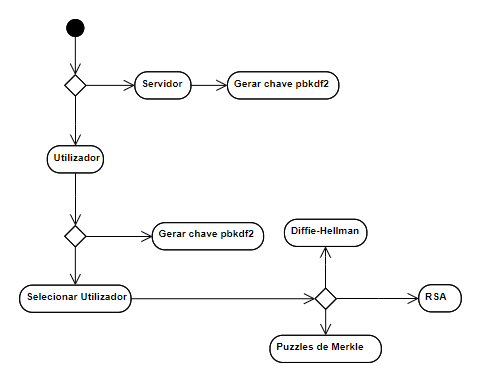
\includegraphics[scale=0.9]{img/atividadessi.png}\newline\caption{Figura 1.1}\end{center}


\newline\begin{center}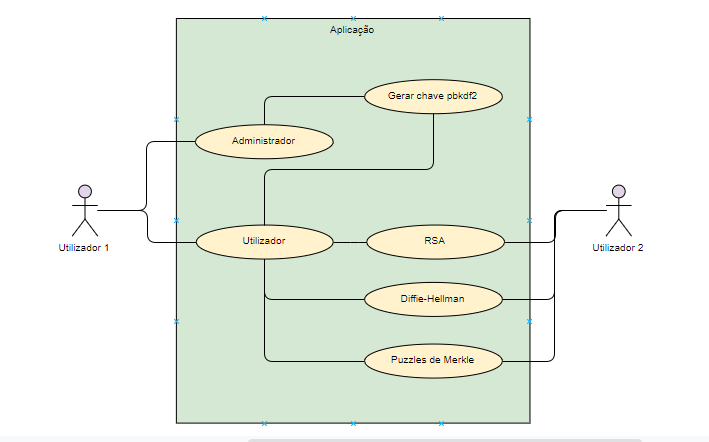
\includegraphics[scale=0.9]{img/casosdeusosi.png}\newline\caption{Figura 1.2}\end{center}



\section{Conclusões}
\label{chap3:sec:concs}
A implementação dos diagramas apresentados neste capítulo demonstram a solidez do projeto elaborado e fornecem uma descrição bastante detalhada do funcionamento do sistema desenvolvido.